%------------------------------------------------

\begin{fullwidth}
High-quality data is essential to most modern development research.
Many research questions require the team to collect original data,
because no source of publicly available data measures the
Many research questions require novel data,
because no source of publicly available data addresses the
inputs or outcomes of interest for the relevant population.
Data acquisition can take many forms, including:
primary data generated through surveys;
private sector partnerships granting access to new data sources, such as administrative and sensor data;
digitization of paper records, including administrative data; web scraping;
primary data capture by unmanned aerial vehicles or other types of remote sensing;
or novel integration of various types of datasets, e.g. combining survey and sensor data.
Much of the recent push toward credibility in the social sciences has focused on analytical practices.
However, credible development research often depends, first and foremost, on the quality of the raw data.
For data work to be reproducible,
in the sense that other researchers would be able to make
equally informed decisions about analytical choices,
the data acquisition process must be clearly and carefully documented.

This chapter covers data acquisition,
special considerations for generating high-quality survey data,
and protocols for safely and securely handling confidential data.
This chapter covers reproducible data acquisition,
special considerations for generating high-quality survey data,
and protocols for safely and securely handling confidential data.
The first section discusses reproducible data acquisition:
how to establish and document your right to use the data.
This applies to all development datasets that are not publicly available,
whether collected for the first time through surveys or sensors or acquired through a unique partnership.
The second section goes into detail on data acquisition through surveys,
as this process is typically more involved than acquisition of secondary data,
and has more in-built opportunities for quality control.
It provides detailed guidance on the electronic survey workflow,
from questionnaire design to programming and monitoring data quality.
We conclude with a discussion of safe data handling,
providing guidance on how to receive, transfer, store, and share confidential data.
Secure file management is a basic requirement to comply with the legal and
ethical agreements that allow  access to personal information for research purposes.


\end{fullwidth}

\section{Acquiring data}
Clearly establishing and documenting data access is critical for reproducible research.
This section provides guidelines for receiving data from development partners,
establishing data ownership,
and documenting the research team's right to use the data.

It is the researchers' responsibility to respect the rights
of people who own the data and the people who are described by it;
but also to make sure that information is as available and accessible as possible.
These twin responsibilities can and do come into tension,
so it is important to be fully informed about what other researchers are doing
and to fully inform other researchers of what you are doing.
Writing down and agreeing to specific details is a good way of doing that.

\subsection{Receiving data from development partners}

Research teams granted access to existing data may receive that data in a number of different ways.
You may receive access to an existing server,
or physical access to extract certain information,
or a one-time data transfer.
In all cases, you must take action to ensure
that data is transferred through
secure channels so that confidentiality is not compromised.
See the section \textit{Handling data securely} later in this chapter for how to do that.
Keep in mind that compliance with ethical research standards may
in some cases require a stricter level of security than initially proposed by the partner agency.

At this stage, it is very important to assess
documentation and cataloging of the data and associated metadata.
It is not always clear what pieces of information will jointly constitute a ``dataset'',
and many of the datasets you receive will not be organized for research.
You should always retain the original data exactly as received
alongside a copy of the corresponding ownership agreement or license.
You should make a simple ``readme'' document noting the date of receipt,
the source and recipient of the data,
and a brief description of each file received.
All too often data will be provided as vaguely-named spreadsheets,
or digital files with non-specific titles,
and documentation will be critical for future access and reproducibility.
Eventually, you will want to make sure that you are creating a set of documents
that can be properly submitted to a data catalog and given a reference and citation.
The metadata -- documentation about the data -- is critical for future use of the data.
Metadata should include documentation of how the data was created,
what they measure, and how they are to be used.
In the case of survey data, this includes the survey instrument and associated manuals;
the sampling protocols and field adherence to those protocols, and any sampling weights;
what variable(s) uniquely identify the dataset(s), and how different datasets can be linked;
and a description of field procedures and quality controls.
DIME uses as a standard the Data Documentation Initiative (DDI), which is supported by the
World Bank's Microdata Catalog.\sidenote{\url{https://microdata.worldbank.org}}

As soon as the desired pieces of information are stored together,
think about which ones are the components of what you would call a dataset.
Often, when you are recieving ``data'' from a partner,
even highly-structured materials such as registers or records
are not, as recieved, equivalent to a research dataset,
and require initial cleaning, restructuring, or recombination
to reach the stage we would consider a raw research dataset.
This is as much an art than a science:
you want to keep information together that is best contextualized together,
but you also want to information granular as much as possible,
particularly when there are varying units of observation.
There usually won't be a single correct way to answer this question,
and the research team will need to decide how the materials recieved.
Soon, you will begin to build datasets from this set of information,
and these will become your original raw data,
which will be the material published, released, and cited as your raw dataset.
These first datasets created from the recieved materials
are the objects you need to catalog, release, and license.
Now is a good time to being assessing disclosure risk
and/or seek publication licenses in collaboration with data providers,
while you are in close contact with them.

\subsection{Data ownership}
Except in the case of primary surveys funded by the research team,
the data is typically not owned by the research team.
Rather, they must enter into data licensing agreements
to access the data and publish research outputs based on it.
These agreements should make clear from the outset whether the
research team can make the original data, any portion thereof, or derivatives\sidenote{
	\textbf{Derivatives} of data can be indicators, aggregates,
	visualizations etc. created from the original data.}
of the data, public.

Data ownership\sidenote{need to add DIME Wiki page} can sometimes be challenging to establish,
as various jurisdictions have differing laws regarding data and information,
and the research team may have their own information regulations.
In some, data is implicitly owned by the people who it is about.
In others, it is owned by the people who collected it.
In still more, it is highly unclear and there are varying norms.
The best approach is always to consult with a local partner,
and enter into specific legal agreements establishing ownership,
access, and publication rights.
This is particularly critical where confidential data is involved
-- that is, when people are disclosing information to you
that you could not obtain simply by observation or through public records.

For original data generated by the research team, such as survey data,
it is important to clarify up front who owns the data,
and who will have access to it.
These details need to be shared with respondents when they are offered the opportunity
to consent to participate in the study.
If the research team is not collecting the data directly --
for example, if a government, private company, or research partner is doing the data collection --
make sure that you have an explicit agreement
about who owns the resulting data.
The contract for data collection should include specific terms
as to the rights and responsibilities of each stakeholder.
It must clearly stipulate which party owns the data produced,
and that the research team maintains full intellectual property rights.
The contract should also explicitly indicate that the contracted firm
is responsible for protecting respondent privacy,
that the data collection will not be delegated to any third parties,
and that the data will not be used by the firm or subcontractors for any purpose not expressly stated in the contract,
before, during or after the assignment.
The contract should also stipulate that the vendor is required to comply with
ethical standards for social science research,
and adhere to the specific terms of agreement with the relevant
Institutional Review Board (IRB)\sidenote{
	\url{https://dimewiki.worldbank.org/IRB\_Approval}}
or applicable local authority.
Finally, it should include policies on reuse, storage, and retention or destruction of data.

Research teams that generate their own data must also consider data ownership downstream,
the terms they will use to release that data to other researchers or to the general public.
Will the team publicly release the data in full (removing personal identifiers)?
Would the team be okay with it being stored on servers anywhere in the world,
even ones that are owned by corporations or governments in other countries?
Would the team prefer to decide permission on a case-by-case basis, dependent on specific proposed uses?
Would the team expect that users of your data cite you or give you credit,
or require users in turn to release
their derivative datasets or publications under similar licenses?
Whatever your answers are to these questions,
make sure the agreement or contract
you use to acquire the data
and the license you issue to accompany its release
specifically details those requirements.

\subsection{Data licensing}
Data licensing is the formal act of the dataset owner
giving some data rights to a specific user,
while retaining ownership of the dataset.
If you are not the owner of the dataset you want to analyze,
you must enter into a licensing agreement to access it for research purposes.
Similarly, when you own a dataset,
you must consider whether you will make the dataset accessible to other researchers,
and what terms-of-use you require.

If the research team requires access to existing data for novel research,
terms of use should be agreed on with the data owner,
typically through a data licensing agreement\sidenote{need to add a DIME wiki page}.
Keep in mind that the data owner is likely not highly familiar
with the research process, and therefore may be surprised
at some of the things you want to do if you are not clear up front.
You will typically want intellectual property rights to all research outputs developed used the data,
a license for all uses of derivative works, including public distribution
(unless ethical considerations contraindicate this).
This is important to allow the research team to store, catalog, and publish, in whole or in part,
either the original licensed dataset or datasets derived from the original.
Make sure that the license you obtain from the data owner allows these uses,
and that you consult with the owner
if you foresee exceptions with specific portions of the data.

The World Bank has a template Data License Agreement which DIME follows.\sidenote{
  \url{https://dimewiki.worldbank.org/Data_License_Agreement}}
The template specifies the specific objectives of the data sharing,
and whether the data can be used only for the established purpose or for other objectives
consistent with the mandates of the signatory organizations.
It establishes classifies the data into four access categories, depending on who can access it, and whether case-by-case authorization is needed.
The data provider may impose similar restrictions to sharing derivative works and any or all of the metadata.
The template also specifies the required citation for the data.
While you do not need to use the World Bank's template or its categories if you do not work on a World Bank project,
we still think it is important that you use this information in two ways.
First, while you do not have to use the World Bank's template,
make sure to base your Data License Agreement using some template.
Second, we strongly recommend you to categorize using the categories above,
or some variation of it.
Then you should have different procedures for each category,
or use one procedure appropriate for the strictest category for all your data.
In addition to what we are suggesting here,
the data provider you work with may impose similar restrictions to sharing derivative works
and any or all of the metadata.

%------------------------------------------------
\section{Collecting data using electronic surveys}
In this section, we detail specific considerations
for acquiring high-quality data through surveys.
There are many survey software options available to researchers,
and the market is rapidly evolving.
There are also many excellent resources on questionnaire design and field supervision,
but few covering the particular challenges and opportunities presented by electronic surveys.
Therefore, we focus on specific workflow considerations for digitally-collected data,
and on basic concepts rather than software-specific tools.
If you are collecting data directly from the research subjects yourself,
you are most likely designing and fielding an electronic survey.
These types of data collection technologies
have greatly accelerated our ability to bring in high-quality data
using purpose-built survey instruments,
and therefore improved the precision of research.
At the same time, electronic surveys create new pitfalls to avoid.
Programming surveys efficiently requires a very different mindset
than simply designing them in word processing software,
and ensuring that they flow correctly and produce data
that can be used in statistical software requires careful organization.
This section will outline the major steps and technical considerations
you will need to follow whenever you field a custom survey instrument,
no matter the scale.

\subsection{Developing a data collection instrument}

A well-designed questionnaire results from careful planning,
consideration of analysis and indicators,
close review of existing questionnaires,
survey pilots, and research team and stakeholder review.
There are many excellent resources on questionnaire design,
such as from the World Bank's Living Standards Measurement Survey.\cite{glewwe2000designing}
The focus of this section is the design of electronic field surveys,
often referred to as Computer Assisted Personal Interviews (CAPI).\sidenote{
  \url{https://dimewiki.worldbank.org/Computer-Assisted\_Personal\_Interviews\_(CAPI)}}
Although most surveys are now collected electronically, by tablet, mobile phone or web browser,
\textbf{questionnaire design}\sidenote{
  \url{https://dimewiki.worldbank.org/Questionnaire\_Design}}
  \index{questionnaire design}
(content development) and \textbf{questionnaire programming}\sidenote{
  \url{https://dimewiki.worldbank.org/Questionnaire\_Programming}}
(functionality development) should be seen as two strictly separate tasks.
Therefore, the research team should agree on all questionnaire content
and design a version of the survey on paper
before beginning to program the electronic version.
This facilitates a focus on content during the design process
and ensures teams have a readable, printable version of their questionnaire.
Most importantly, it means the research, not the technology,
drives the questionnaire design.

We recommend this approach because an easy-to-read paper questionnaire
is very useful for training data collection staff,
because it focuses on the survey content and structure
before diving into the technical components.
It is much easier for enumerators to understand
the range of possible participant responses
and how to handle them correctly on a paper survey than on a tablet,
and it is easier to translate that logic to digital functionality later.
Finalizing this version of the questionnaire before beginning any programming
avoids version control concerns that arise from concurrent work
on paper and electronic survey instruments.
Finally, a readable paper questionnaire is a necessary component of data documentation,
since it is difficult to work backwards from the survey program to the intended concepts.

The workflow for designing a questionnaire will feel much like writing an essay, or writing pseudocode:
begin from broad concepts and slowly flesh out the specifics.\sidenote{
  \url{https://dimewiki.worldbank.org/wiki/Questionnaire_Design}}
It is essential to start with a clear understanding of the
\textbf{theory of change}\sidenote{
  \url{https://dimewiki.worldbank.org/Theory\_of\_Change}}
and \textbf{research design} for your project.
The first step of questionnaire design is to list key outcomes of interest,
as well as the main covariates to control for and any variables needed for the specific research design.
The ideal starting point for this is a \textbf{pre-analysis plan}.\sidenote{
  \url{https://dimewiki.worldbank.org/Pre-Analysis\_Plan}}

Use the list of key outcomes to create an outline of questionnaire \textit{modules}.
Do not number the modules; instead use a short prefix
as numbers quickly get outdated when modules are reordered.
For each module, determine if the module is applicable to the full sample,
or only to specific respondents,
and whether or how often the module should be repeated.
A few examples:
a module on maternal health only applies
to households with a woman who has children,
a household income module should be answered
by the person responsible for household finances,
and a module on agricultural production
might be repeated for each crop the household cultivated.
Each module should then be expanded
into specific indicators to observe in the field.\sidenote{
  \url{https://dimewiki.worldbank.org/Literature\_Review\_for\_Questionnaire}}
At this point, it is useful to do a  \textbf{content-focused pilot}\sidenote{
  \url{https://dimewiki.worldbank.org/Piloting\_Survey\_Content}}
of the questionnaire.
Doing this pilot with a pen-and-paper questionnaire encourages more significant revisions,
as there is no need to factor in time costs of re-programming,
and as a result improves the overall quality of the survey instrument.
Questionnaires must also include ways to document the reasons for \textbf{attrition} and
treatment \textbf{contamination}.\index{attrition}\index{contamination}
These are essential data components for completing CONSORT records,
a standardized system for reporting enrollment, intervention allocation, follow-up,
and data analysis through the phases of a randomized trial.\cite{begg1996improving}

A comprehensive survey pilot is a critical stage in survey design.\sidenote{
	\url{https://dimewiki.worldbank.org/Survey\_Pilot}} 
The pilot must be done out-of-sample,
but in a context as similar as possible to the study sample.
The survey pilot includes three steps: 
a \textbf{pre-pilot}, a \textbf{content-focused pilot}, and a \textbf{data-focused pilot}.\sidenote{
	\url{https://dimewiki.worldbank.org/wiki/Structuring\_a\_Survey\_Pilot}} 
The first step is a pre-pilot. 
The pre-pilot is a qualitative exercise, done early in the questionnaire design process.
The objective is to answer broad questions about how to measure key outcome variables,
and gather qualitative information relevant to any of the planned survey modules.  
A pre-pilot is particularly important when designing new survey instruments.
The second step is a content-focused pilot\sidenote{
  \url{https://dimewiki.worldbank.org/Piloting\_Survey\_Content}}.
The objectives at this stage are to improve the structure and length of the questionnaire,
refine the phrasing and translation of specific questions,
and confirm coded response options are exhaustive.\sidenote{
	\url{https://dimewiki.worldbank.org/index.php?title=Checklist:\_Refine\_the\_Questionnaire\_(Content)}}
In addition, it is an opportunity to test and refine all survey protocols,\sidenote{
	\url{https://dimewiki.worldbank.org/wiki/Piloting\_Survey_Protocols}}
such as how units will be sampled or pre-selected units identified.
The content-focused pilot is best done on pen and paper, before the questionnaire is programmed,
because changes at this point may be deep and structural,
which are hard to adjust in code.
The final stage is a data-focused pilot.
The objective at this stage is to refine the questionnaire programming; this is discussed in more detail in the following section.\sidenote{
	\url{https://dimewiki.worldbank.org/wiki/Timeline\_of\_Survey\_Pilot}}


\subsection{Designing surveys for electronic deployment}
Once the team is satisfied with the content and structure of the survey,
it is time to move on to implementing it electronically.
Electronic data collection has great potential
to simplify survey implementation and improve data quality.
Electronic questionnaires are typically created
in a spreadsheet (e.g. Excel or Google Sheets)
or a software-specific form builder,
all of which are accessible even to novice users.\sidenote{
  \url{https://dimewiki.worldbank.org/Questionnaire\_Programming}}
We will not address software-specific form design in this book;
rather, we focus on coding conventions that are important to follow
for electronic surveys regardless of software choice.\sidenote{
  \url{https://dimewiki.worldbank.org/SurveyCTO\_Coding\_Practices}}
Survey software tools provide a wide range of features
designed to make implementing even highly complex surveys
easy, scalable, and secure.
However, these are not fully automatic:
you need to actively design and manage the survey.
Here, we discuss specific practices that you need to follow
to take advantage of electronic survey features
and ensure that the exported data
is compatible with your statistical software.

From a data perspective, questions with pre-coded response options
are always preferable to open-ended questions.
The content-based pilot is an excellent time to ask open-ended questions
and refine fixed responses for the final version of the questionnaire --
do not count on coding up lots of free text after a full survey.
Coding responses helps to ensure that the data
will be useful for quantitative analysis.
Two examples help illustrate the point.
First, instead of asking ``How do you feel about the proposed policy change?'',
use techniques like \textbf{Likert scales}\sidenote{
  \textbf{Likert scale:} an ordered selection of choices indicating the respondent's level of agreement or disagreement with a proposed statement.}.
Second, if collecting data on medication use or supplies, you could collect:
the brand name of the product; the generic name of the product; the coded compound of the product;
or the broad category to which each product belongs (antibiotic, etc.).\sidenote{
  See \citet{wafula2017examining} for an example.}
All four may be useful for different reasons,
but the latter two are likely to be the most useful for rapid data analysis.
The coded compound requires providing a translation dictionary to field staff,
but enables automated rapid recoding for analysis with no loss of information.
The generic class requires agreement on the broad categories of interest,
but allows for much more comprehensible top-line statistics and data quality checks.
Rigorous field testing is required to ensure that answer categories are comprehensive;
however, it is best practice to include an \textit{other, specify} option.
Keep track of those responses in the first few weeks of field work.
Adding an answer category for a response frequently showing up as \textit{other} can save time,
as it avoids extensive post-coding.

It is essential to name the fields in your questionnaire
in a way that will also work in your data analysis software.
Most survey programs will not enforce this by default,
since limits vary across statistical software,
and survey software will encourage you
to use long sentences as question labels
and detailed descriptions as choice options.
This is what you want for the enumerator-respondent interaction,
but you should already have analysis-compatible labels programmed in the background
so the resulting data can be rapidly imported in analytical software.
There is some debate over how exactly individual questions should be identified:
formats like \texttt{hq\_1} are hard to remember and unpleasant to reorder,
but formats like \texttt{hq\_asked\_about\_loans} quickly become cumbersome.
We recommend using descriptive names with clear prefixes so that variables
within a module stay together when sorted alphabetically.\sidenote{
  \url{https://dimewiki.worldbank.org/Variable_Names}}
Variable names should never include spaces or mixed cases
(we prefer all-lowercase naming).
Take special care with the length: very long names will be cut off in some softwares,
which could result in a loss of uniqueness and lots of manual work to restore compatibility.
We further discourage explicit question numbering,
at least at first, as it discourages re-ordering questions,
which is a common recommended change after the pilot.
In the case of follow-up surveys, numbering can quickly become convoluted,
too often resulting in uninformative variables names like
\texttt{ag\_15a}, \texttt{ag\_15\_new}, \texttt{ag\_15\_fup2}, and so on.

\subsection{Programming electronic questionnaires}

The starting point for questionnaire programming
is a complete paper version of the questionnaire,
piloted for content and translated where needed.
Doing so reduces version control issues
that arise from making significant changes
to concurrent paper and electronic survey instruments.
Changing structural components of the survey
after programming has been started
often requires the coder to substantially re-work the entire code.
This is because the more efficient way to code surveys is non-linear.
When programming, we do not start with the first question and proceed through to the last question.
Instead, we code from high level to small detail,
following the same questionnaire outline established at design phase.
The outline provides the basis for survey pseudocode,
allowing you to start with high level structure and work down to the level of individual questions.
This will save time and reduce errors,
particularly where sections or fields
are interdependent or repeated in complex ways.

Electronic surveys are more than simply
a paper questionnaire displayed on a mobile device or web browser.
All common survey software allows you to automate survey logic
and include hard or soft constraints on survey responses.
These features make enumerators' work easier,
and they create the opportunity to identify and resolve
data issues in real time,
simplifying data cleaning and improving response quality.
Well-programmed questionnaires should include
most or all of the following features:

\begin{itemize}
  \item{\textbf{Localization}}: the survey instrument should display full-text questions and responses in all potential survey languages, and it should also have English and code-compatible versions of all text and labels.
	\item{\textbf{Survey logic}}: built-in tests should be included for all logic connections between questions, so that only relevant questions appear, rather than relying on enumerators to follow complex survey logic. This covers simple skip codes, as well as more complex interdependencies (e.g., a child health module is only asked to households that report the presence of a child under 5).
	\item{\textbf{Range checks}}: add range checks for all numeric variables to catch data entry mistakes (e.g. \texttt{age} must be less than 120).
	\item{\textbf{Confirmation of key variables}}: require double entry of essential information (such as a contact phone number in a survey with planned phone follow-ups), with automatic validation that the two entries match and rejection and re-entry otherwise.
	\item{\textbf{Multimedia}}: electronic questionnaires facilitate collection of images, video, and geolocation data directly during the survey, using the camera and GPS built into the tablet or phone.
	\item{\textbf{Preloaded data}}: data from previous rounds or related surveys can be used to prepopulate certain sections of the questionnaire, and validated during the survey.
	\item{\textbf{Filtered response options}}: filters reduce the number of response options dynamically (e.g. filtering a ``cities'' choice list based on the state selected).
	\item{\textbf{Location checks}}: enumerators submit their actual location using in-built GPS, to confirm they are in the right place for the interview.
	\item{\textbf{Consistency checks}}: check that answers to related questions align, and trigger a warning if not so that enumerators can probe further (e.g., if a household reports producing 800 kg of maize, but selling 900 kg of maize from their own production).
	\item{\textbf{Calculations}}: make the electronic survey instrument do all math, rather than relying on the enumerator or asking them to carry a calculator.
\end{itemize}

All established survey software include debugging and test options
to correct syntax errors and make sure that
the survey instruments will successfully compile.
This is not sufficient, however, to ensure that the resulting dataset
will load without errors in your data analysis software of choice.
DIME Analytics developed the \texttt{ietestform} command,\sidenote{
  \url{https://dimewiki.worldbank.org/ietestform}}
part of the Stata package \texttt{iefieldkit},
to implement a form-checking routine for \textbf{SurveyCTO},
a proprietary implementation of the open source \textbf{Open Data Kit (ODK)} software.
Intended for use during questionnaire programming and before field work,
\texttt{ietestform} tests for best practices
in coding, naming and labeling, and choice lists.
Although \texttt{ietestform} is software-specific,
many of the tests it runs are general and important to consider regardless of software choice.
To give a few examples, \texttt{ietestform} tests that no variable names exceed
32 characters, the limit in Stata (variable names that exceed that limit will
be truncated, and as a result may no longer be unique).
It checks whether ranges are included for numeric variables.
\texttt{ietestform} also removes all leading and trailing blanks from response lists,
which could be handled inconsistently across software.

The final stage of survey piloting, the data-focused pilot, should be done at this stage (after the questionnaire is programmed).
The objective of this \textbf{data-focused pilot}\sidenote{
  \url{https://dimewiki.worldbank.org/index.php?title=Checklist:\_Refine\_the\_Questionnaire\_(Data)}}
is to validate the programming and export a sample dataset.
Significant desk-testing of the instrument is required to debug the programming
as fully as possible before going to the field.
It is important to plan for multiple days of piloting,
so that any debugging or other revisions to the electronic survey instrument
can be made at the end of each day and tested the following, until no further field errors arise.
The data-focused pilot should be done in advance of enumerator training.

\subsection{Finalizing data collection}

When all data collection is complete,
the survey team should prepare a final field report,
which should report reasons for any deviations between the original sample and the data collected.
Identification and reporting of \textbf{missing data} and \textbf{attrition}
is critical to the interpretation of survey data.
It is important to structure this reporting in a way that not only
groups broad rationales into specific categories
but also collects all the detailed, open-ended responses
to questions the field team can provide for any observations that they were unable to complete.
This reporting should be validated and saved alongside the final raw data, and treated the same way.
This information should be stored as a dataset in its own right
-- a \textbf{tracking dataset} -- that records all events in which survey substitutions
and attrition occurred in the field and how they were implemented and resolved.\sidenote{
  See \citet{kondylis2020demand} for an example.}


%------------------------------------------------
\section{Handling data securely}

All confidential data must be handled in such a way that only people specifically
approved by an Institutional Review Board (IRB)
are able to access the data.
Data can be confidential for multiple reasons; two 
very common reasons are that the data contains personally identifiable information (PII)\sidenote{
  \url{https://dimewiki.worldbank.org/Personally\_Identifiable\_Information\_(PII)}}
or that the data owner has specified restricted access.


\subsection{Encryption}

\index{encryption}\textbf{Data encryption} is a group of methods that ensure that files are unreadable
even if laptops are stolen, servers are hacked,
or unauthorized access to the data is obtained in any other way.\sidenote{
  \url{https://dimewiki.worldbank.org/Encryption}}
Proper encryption is central to secure data handling, and can rarely be condensed into a single method,
as the data will travel through many servers, devices, and computers
from the source of the data to the final analysis.
Encryption should be seen as a system
that is only as secure as its weakest link.
This section recommends a streamlined workflow,
so that it is easy as possible to make sure
the weakest link is still sufficiently secure.

Data that has been encrypted is made readable again using decryption,
and decryption requires a password or a key.
Encryption make data files completely unusable to anyone without the specific decryption key,
which is a higher level of security than password-protection.
It is never secure to share passwords or keys by email,
WhatsApp or other insecure modes of communication;
instead, use a secure password manager.\sidenote{
	\url{https://lastpass.com} or \url{https://bitwarden.com}
	among many other. See the DIME Analytics guide to password managers
  on the DIME Standards site: \url{https://github.com/worldbank/dime-standards/}}
In addition to providing a way to securely share passwords,
password managers also provide a secure location
for long term storage of passwords and keys,
whether they are shared or not.
Make sure you store your keys with descriptive names,
as they will be needed over the lifetime of a project.

There are two main types of encryption algorithms and they are called
\textbf{symmetric encryption}\sidenote{
	\url{https://dimewiki.worldbank.org/Encryption\#Symmetric\_Encryption}}
and \textbf{asymmetric encryption}\sidenote{
	\url{https://dimewiki.worldbank.org/Encryption\#Asymmetric\_Encryption}}.
The only difference you need to know is that the same key is used to both
encrypt and decrypt the data in symmetric encryption,
while in asymmetric encryption,
one key in a key pair is used to encrypt the data,
and the other key in the same pair is used to decrypt it.
We will show how this difference can be utilized for different use cases common in research.


Additionally, there are two contexts for encryption you should be aware of;
\textbf{encryption-in-transit}\sidenote{
	\url{https://dimewiki.worldbank.org/Encryption\#Encryption\_in\_Transit}}
and \textbf{encryption-at-rest}\sidenote{
	\url{https://dimewiki.worldbank.org/Encryption\#Encryption\_at\_Rest}}.
Encryption-in-transit protects your data when in transit over the internet.
It is easy to implement encryption-in-transit such that no input from the user is required,
since the server and browser can keep track of the key for the short duration of the connection.
All well-established data transfer services have this implemented and you rarely have to worry about it.
However, if you are setting up a custom solution,
it is important that you verify that it use encryption-in-transit,
as without it, your data and credentials are very vulnerable.
Encryption-at-rest protects your data when it is stored somewhere,
for example on a server or on your computer.
In contrast to encryption-in-transit,
you as a user, need to keep track of the key.
Only people listed on your IRB should be allowed to have access to this file.

Many data-sharing and data-storage software providers will promote their services
by advertising on-the-fly encryption and decryption.
However, this is often only encryption-in-transit and not encryption-at-rest.
Sometimes on-the-fly encryption involves encryption-at-rest,
but then you have to verify how the encryption key is handled
as individuals who are not approved by your IRB,
such as tech support personnel,
server administrators, and other third-party staff
are not allowed to have access to the key.
It is possible, in some enterprise versions of data sharing software,
to set up appropriately secure on-the-fly encryption.
However, that setup is advanced, and you should never trust it
unless a cybersecurity expert within your organization
has specified what it can be used for.
In all other cases you should follow the steps laid out in this section,
where you set up your own encryption
where you are in full control of who has access to the key.


\subsection{Storing data securely}
% doesn't cover 'big' data
The first thing you need to do before planning how to securely receive data,
is to plan how to securely store data after you have received it.
Typically, you want to store your data so that you can decrypt and access it,
interact with it and then decrypt it again.
That is a perfect use case for \textbf{symmetric encryption}
where the same key is used to both encrypt and decrypt your files.
Think of this as a physical safe where you have one key
used to both add content and access content.

The equivalent to a safe in secure data storage is an encrypted folder,
which you can set up using, for example, VeraCrypt.\sidenote{
	\url{https://www.veracrypt.fr} described at
	\url{https://github.com/worldbank/dime-standards}}
You can interact with files in an encrypted folder, and modify themlike any unencrypted file,
as long as you have the key.
This is an implementation of encryption-at-rest.
There is absolutely no way to restore your data if you were to lose your key,
so we cannot stress enough the importance of using a password manager,
or equally secure solution, to store these encryption keys.

It is becoming more and more common that development research
is done on data set that is too big to store on a regular computer,
and instead the data is stored and processed in a cloud environment.
There are many available cloud storage solutions
and you need to understand how the data is encrypted and how the keys are handled.
This is likely another case where a regular research team will have to ask a cybersecurity expert.
After someone have helped you to set up a secure cloud storage,
if you were to download a sample of the data --
for example to develop your code on --
then you need to remember to encrypt the data when stored on your computer.

\subsection{Collecting data securely in the field}

All common data collection software will automatically encrypt
all data in transit (i.e., upload from field or download from server).
However, it is also necessary to ensure that confidential data
are protected when stored on a server owned by the data collection software provider.
You should not assume that your data is encrypted-at-rest by default.
In most data collection platforms,
encryption-at-rest needs to be explicitly enabled and operated by the user.

When collecting data you want the tablets or the browsers used for data collection
to be able to encrypt all information before submitting it to the server.
At the same time you do not want those devices to have any way of decrypting already submitted data.
This is a perfect use case for \textbf{asymmetric encryption}
where there are two keys, forming a public/private key pair.
The public key can safely be sent to all tablets or browsers so it can be used for encrypting the data before it is submitted to a server.
Only the private key in the same key pair can then be used to decrypt that data
so it can be accessed after it has been received.
The private key should be kept secret and should not be shared with anyone not listed on the IRB.
Again, you must store the key pair in a secure location,
such as a secure note in a password manager,
as there is no way to access your data if the private key is lost.\sidenote{
  DIME guidelines for encryption in SurveyCTO/ODK are part of the DIME Standards:
  \url{https://github.com/worldbank/dime-standards/}}

Data encrypted this way can securely pass
through a server accessible by the data collection software provider
or by your local IT team,
and you should never decrypt it until it is downloaded on your computer.
If your data collection service allows you to browse data in the browser,
then the encryption is only implemented correctly if you are asked for the key each time.

Finally, the data security standards that apply
when receiving confidential data from the field
also apply when transferring confidential data to the field.
In some survey software,
you can use the same encryption that allows you to receive data securely
from the field, to also send confidential data,
such as an identifying list of respondents, to the field.

\subsection{Receiving or sharing data securely}

If you receive confidential data from a partner organization
or share confidential data with your research team over the internet,
it must always be encrypted.
The best practice is to reduce the amount of confidential data
that is shared or transfer.
If you do not need the confidential information, you will simplify your workflow
by acquiring or sharing data without any confidential information in the first place.
Removing confidential information, for example through de-identifying the data
(which we will discuss in detail in Chapter 5), should always be your first preference.

Usually we need to deal with confidential data at some point in the project,
and then the second best practice is create two versions of your data.
One version of your data will still have the confidential information,
and it will need to be encrypted at all times.
This version should only be used when the confidential information is actually needed.
In the second version of your data all confidential data should be removed.
This version does not have to be encrypted
and should be what you use on a day-to-day basis.

The most common reason data is confidential is that it includes personal identifiers.
Removing identifying information is called de-identification,
and we will discuss how to do that in the next chapter.
De-identifying the data at the earliest possible opportunity
will simplify the workflow without compromising data security,
as de-identified data no longer needs to be encrypted.
Another method to protect confidential data is to aggregate the data,
meaning that sums and averages of group of observations are calculated
and only those numbers are reported.
Any of these techniques can be used either before the data is shared with the research team,
or when creating the second non-confidential version of the data set to be used in the analysis.
If confidential information is directly required for the analysis,
it will be necessary to keep at least a subset of the data encrypted through the data analysis process.

There are multiple options for sharing encrypted data.
If you need to collaborate on a confidential data set
then you can create an encrypted folder, for example using VeraCrypt (as described above).
An encrypted folder can safely be shared using insecure modes of communication
such as email or third-party syncing services,
as long as you only share the key
using a secure service like a password manager.
Anyone who has access to both the encrypted folder \textit{and} the encryption key
can read and collaborate on the encrypted file.
If you only need a one-time transfer of confidential information,
such as to receive a data set from a partner organization,
then setting up a permanent encrypted folder may be unnecessary.
Instead, for one-time transfers we recommend sending data over password-protected
end-to-end encrypted file sharing services.\sidenote{
	One such service at the time of writing is \url{https://send.firefox.com/}}

\subsection{Backing up original data}
In addition to encrypting your data, you must protect it 
from being accidentally overwritten or deleted.
This is done through a back-up protocol.
Here is an example of such a protocol:

\begin{enumerate}
	\item Create an encrypted folder in your project folder.
	This should be on your computer, and could be in a shared folder.

	\item Download your original data from your data source to that encrypted folder.
	If your data source is a survey and the data was encrypted during data collection,
	then you will need \textit{both} the
	private key used during data collection to be able to download the data,
	\textit{and} the key used when you created the encrypted folder to save it there.
	This your first copy of your raw data, and the copy you will use in your cleaning and analysis.

	\item Create a second encrypted folder on an external drive that you can keep in a secure location.
	Copy the data you just downloaded to this second encrypted folder.
	This is the ``master'' backup copy of the raw data.
	You should never work with this data on a day-to-day basis.
	You should not use the same encrypted folder or the same key as above,
	because if you use the same key and lose the key,
	then you will have lost access to both encrypted folders.
	If you have an physical safe where you can securely store the external drive,
	then you do not need to encrypt the data
	and thereby do not risk losing access by losing an encryption key.

	\item Finally, create a third encrypted folder.
	Either you can create this on your computer and upload it to a long-term cloud storage service (not a sync software),
	or you can create it on	another external hard drive or computer that you then store in a second location,
	for example, at another office of your organization.
	This is the ``golden master'' backup copy of the raw data.
	You should never store the ``golden master'' copy in a synced folder,
	as it would be deleted in the cloud storage if it is deleted on your computer.
	You should also never work with this data;
	it exists only for recovery purposes.
\end{enumerate}

\noindent This handling satisfies the \textbf{3-2-1 rule} described in Chapter 2:
there are two on-site copies of the data and one off-site copy,
so the data can never be lost in case of hardware failure.
%needs wiki page
If you remain lucky, you will never have to access your ``master'' or ``golden master'' copies --
you just want to know it is there, safe, if you one day end up needing it.

\section{Looking ahead}

Once the raw data is completely transferred, securely stored and backed up,
the data acquisition stage, 
summarized in the "Data acquisition workflow" figure, is complete.
This is when the heavy lifting on statistical software starts.
If you think that now you can proceed to analyze your data and answer your project's research questions,
think again.
Before you can do that, you need to check the quality of the data acquired
and make sure you have the right information in the right format.
This proces, which we call data cleaning and processing,
is described in the next chapter.

\begin{fullwidth}
	\begin{figure}
		\centering
		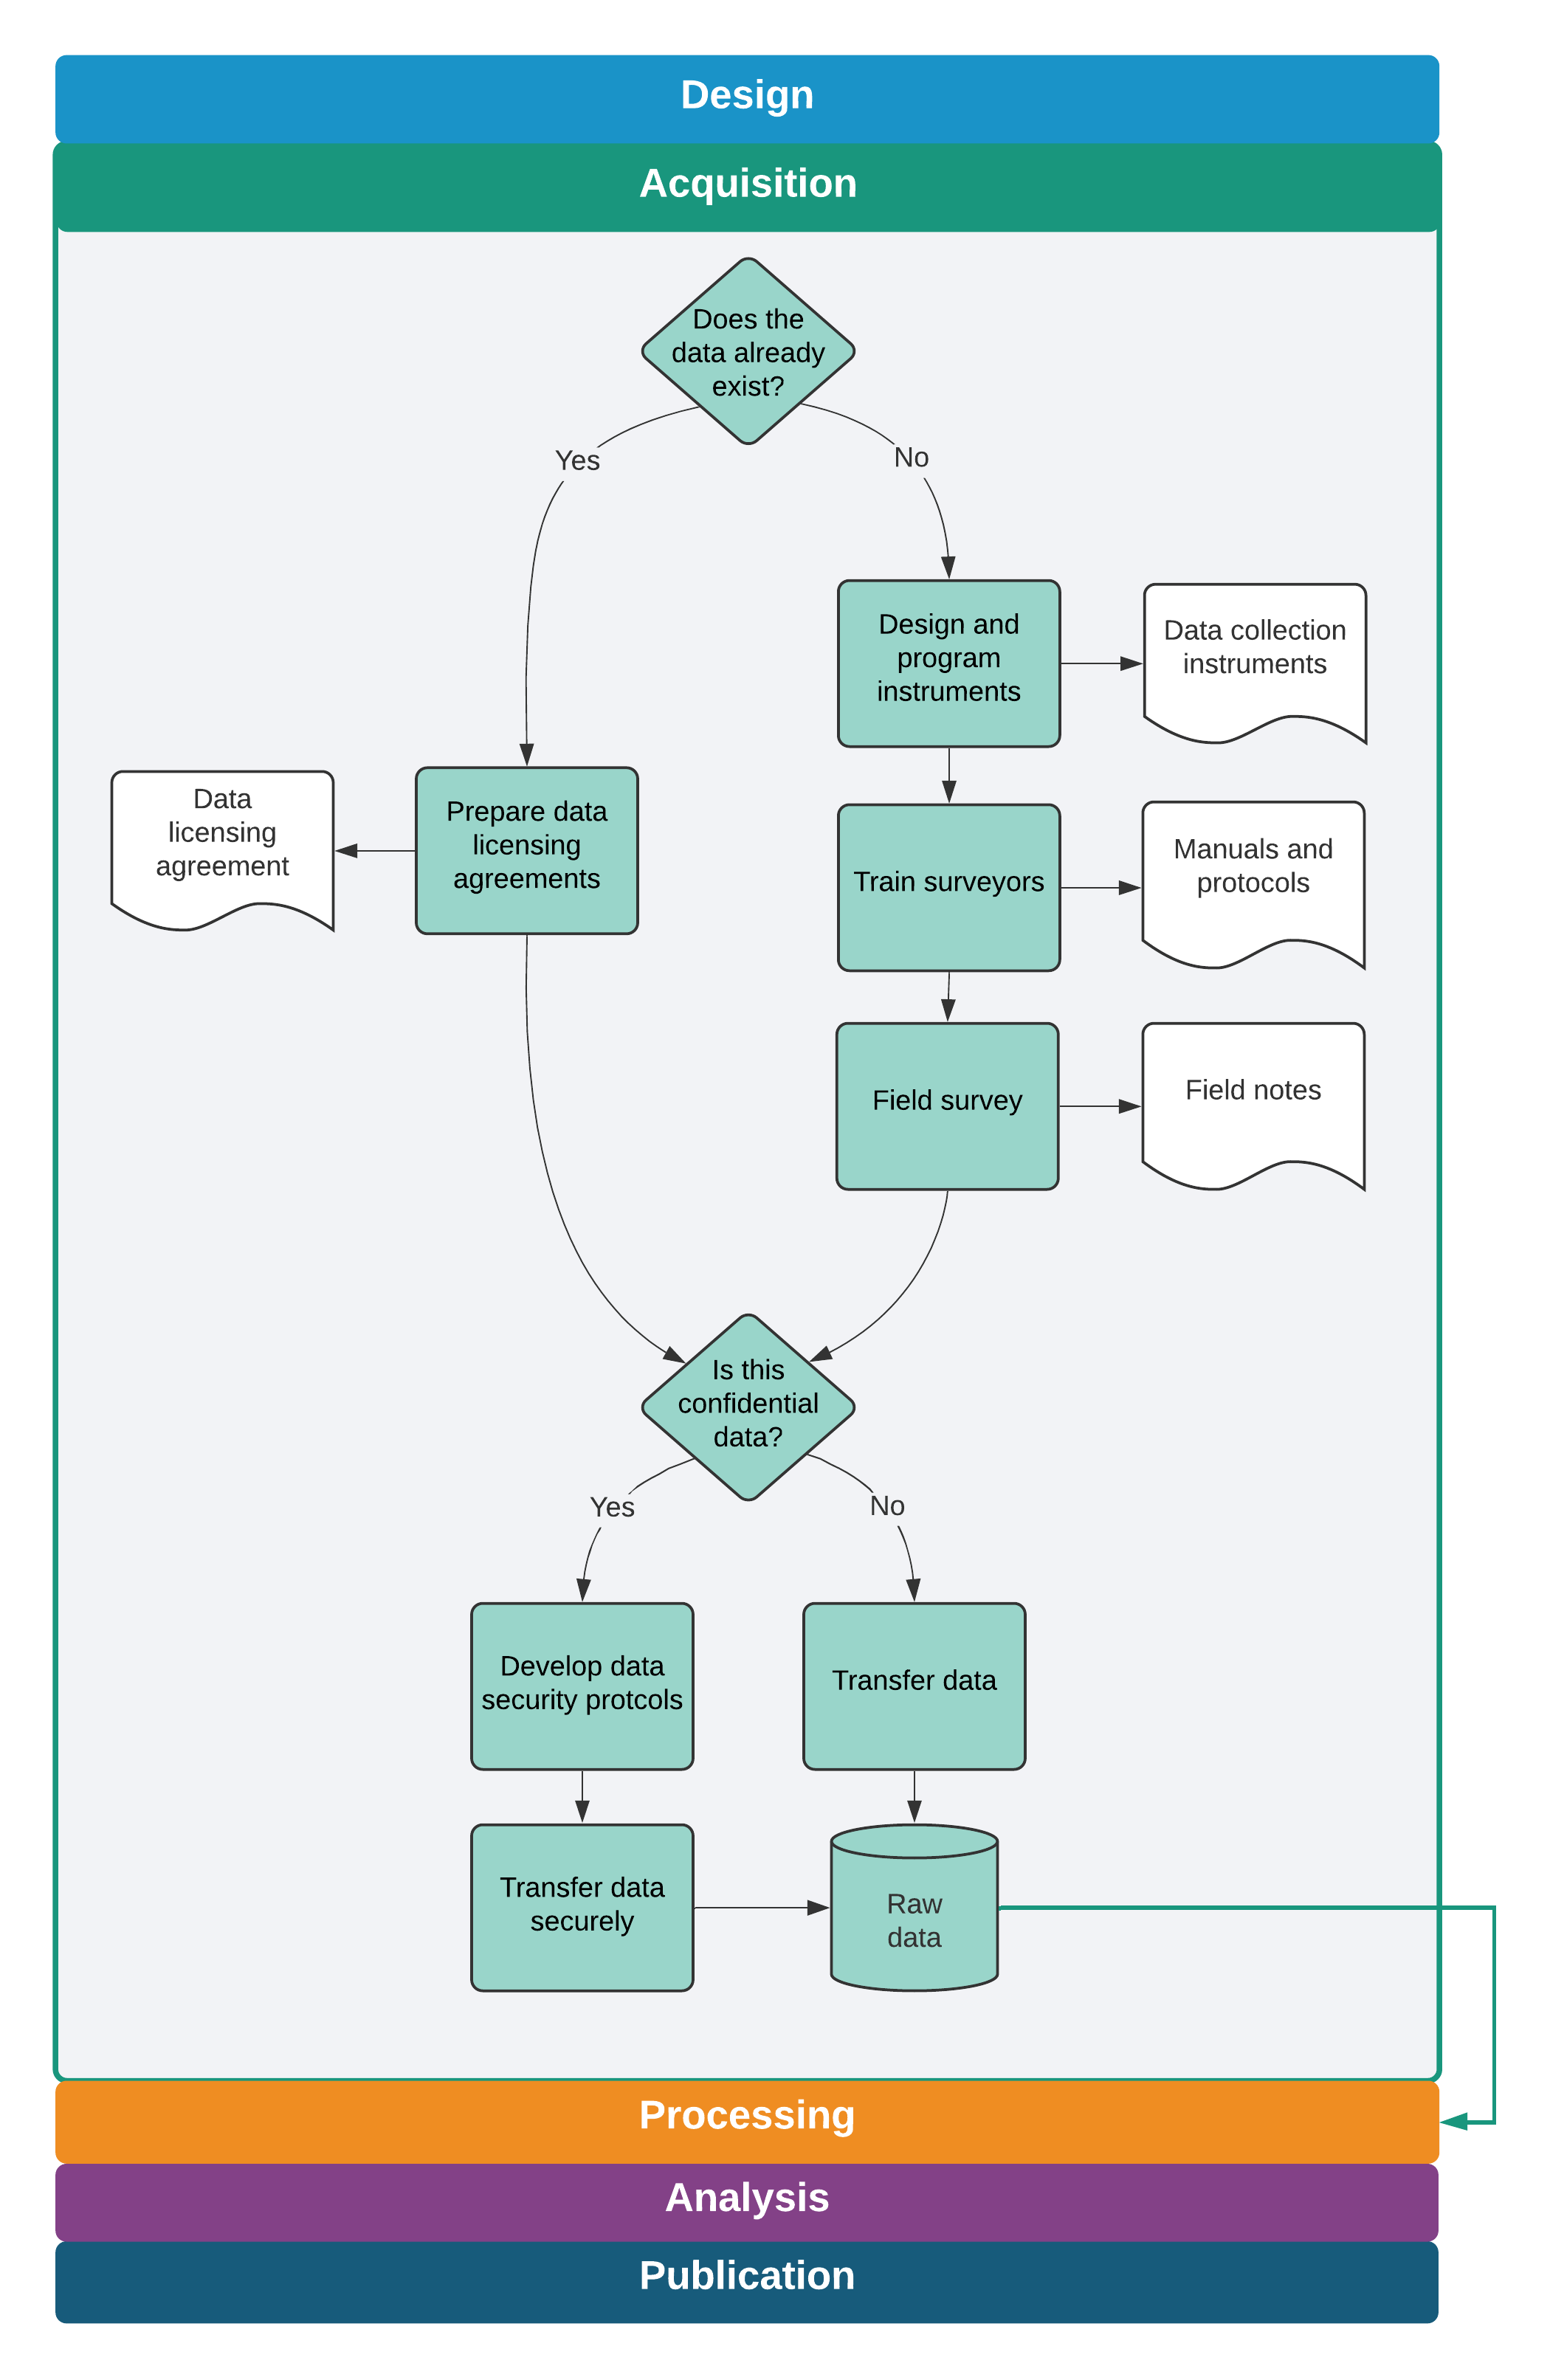
\includegraphics[width=1.5\linewidth]{diagrams/Acquisition}
		\caption{\small Data acquisition workflow}
	\end{figure}
\end{fullwidth}
